%! Author = Saeid Yazdani
%! Date = 1/18/2024

%%%%%%%%%%%%%%%%%%%%%%%%%%%%%%%%%%%%%%%%%%%%%%%%%%%%%%%%%%%%%%%%%%%%%%%%%%%%%%%%


\section{Description of the Target \ac{ATE} Environment}
\label{sec:case-study-target-desc}
%%%%%%%%%%%%%%%%%%%%%%%%%%%%%%%%%%%%%%%%%%%%%%%%%%%%%%%%%%%%%%%%%%%%%%%%%%%%%%%%

\subsection{\acs{DUT} Description}
\label{subsec:dut_description}

The \ac{DUT} under investigation is a prototype of a
modern multicore microcontroller with multiple digital (\ac{DSP} core,
timers, etc. ) and analog peripherals (\acp{ADC}, amplifiers, etc.) with the
following package details:

\begin{itemize}[topsep=8pt,itemsep=4pt,partopsep=4pt, parsep=4pt]

    \item \textbf{Type:} Microcontroller
    \item \textbf{Core Voltage:} \SI{1.3}{\volt}
    \item \textbf{Average Loaded Current:} \SI{550}{\milli\ampere}
    \item \textbf{\ac{I/O} Voltage:} \SI{3.3}{\volt}
    \item \textbf{Package:} \ac{BGA}
    \item \textbf{Pin Count:} 292
    \item \textbf{Pin pitch:} \SI{0.8}{\milli\meter}
    \item \textbf{Physical Dimensions:} \SI{17}{\milli\meter} (L) x \SI{17}{\milli\meter} (W) x \SI{1.7}{\milli\meter} (H)

\end{itemize}

%\subsection{Description of \acs{ATE}'s \acs{DPS} Modules}

\subsection{\acs{DPS} Modules}
\label{ate-and-dps_description}

The \ac{ATE} under investigation is a popular test system throughout
the industry.
Within the \ac{ATE}, standard \ac{DPS} units are used for powering
up to four \acs{DUT}s.
The key features of the installed \ac{DPS} modules are:

\begin{itemize}[topsep=8pt,itemsep=4pt,partopsep=4pt, parsep=4pt]

    \item \textbf{Voltage Range:}
    \SI{0}{\volt} to \SI{10}{\volt} with 12 bits resolution.

    \item\textbf{Current Range:} \SI{0}{\ampere} - \SI{1}{\ampere} per channel.

    \item \textbf{Current Limit:}
    \SI{50}{\milli\ampere} - \SI{1}{\ampere}

\end{itemize}

\subsection{Load Board Description}
\label{load-board_description}

The quad site load board is designed to support testing of up to four
\acp{DUT} simultaneously, as shown in \autoref{fig:villach-load-board-standing}.
The dimensions are \SI{60}{\centi\meter} by \SI{40}{\centi\meter} and layer
count is 32.
In Addition, each \ac{DUT} site is accompanied with a number of
passive and active components such as multiplexer and signal relays to
help with testing.

\begin{figure}[h]
    \centering
    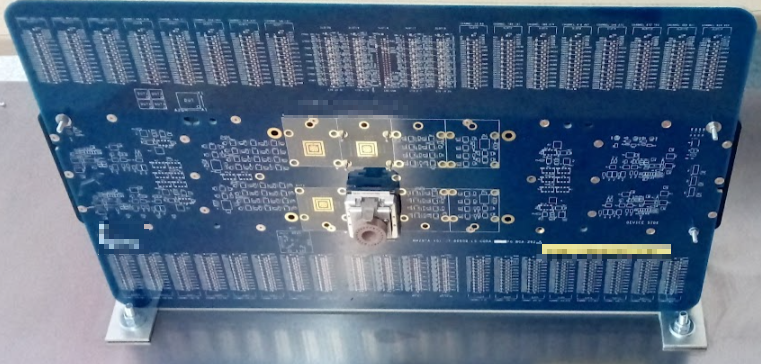
\includegraphics[width=\textwidth]
    {figures/villach-load-board-standing}
    \caption[The Load Board Under Investigation]{
        The load board is under investigation.
    }
    \label{fig:villach-load-board-standing}
\end{figure}

\subsection{Investigation Goals}
\label{subsec:investigation-goals}

\acp{DUT} were affected with unexpected resets, resulting in wasted valuable
test time and delay in the test pipeline.
In such situations, a test engineer might assume the \ac{DUT} is defective and
could overlook the influence of the \ac{ATE} wiring and power supply behavior.

A thorough review of the test system and the used load board unveiled the
causes for the misbehavior and helped with proposing remedies, especially when
the test results indicated the same behavior for different testers of the
same origin and configuration.

Assuming that the \acp{DUT} are not the root cause of the
issue, the investigation focuses on the path from \ac{ATE} to \ac{DUT} which
includes wiring and interconnects, power supply switching behavior, load board
parameters and the test sockets.
